\documentclass[8.01x]{subfiles}
\begin{document}

\chapter{Introduction}

Hello!

These are the notes I've taken, as a student, while taking this course.\\
As such, they may contain errors, and are most certainly incomplete (there's no way you could learn the content of this course from these notes!), and so on. Keep in mind that I'm just a student -- if a reliable source contradicts something in here, that source is most likely correct!

I will use some citations in these notes, which aren't really intended as citations the way you'd use them in a proper scientific paper. Instead, they are used to show where I got the majority of the information for a small part of the notes, in a less strict and more ``relaxed'' way than you would see in a published paper.\\
Wherever there are no citations at all, the source is by default the week's lecture videos and/or other course materials. I will only add citations for external sources (such as other books, web pages etc.) as there would be way too many citations otherwise.

Any unsourced references to ``the book'' or ``the textbook'' is to (of course) the book used by the course: ``Classical Mechanics'' by Peter Dourmashkin.

I write down my thought processes and solutions to homework and exam problems while solving them. I look through them after having read the staff's official solutions (available by going back to the homework after deadline and clicking ``Show answer(s)''); however, unless my answers are incorrect (such that I just got lucky with the green checkmark), I don't really revise them after the fact.\\
Therefore, the official solutions are often neater than mine! I still write these, mostly as a learning tool for myself, though.\\
Feel free to look through them, but be aware that they may be overly convoluted at times!

\chapter{Vector mathematics}

Many quantities in physics can be represented as a single number (a \emph{scalar}): mass, temperature and distance are some examples. However, other quantities - such as force and velocity - have a \emph{direction} as well as a magnitude. These quantities are represented by \emph{vectors}, which are made up of two parts: magnitude (the ``size'' of the vector) and direction.\\
This distinction is what makes up the difference between velocity (a vector) and speed (the \emph{magnitude} of velocity, i.e. a number/scalar that is always either zero or positive). The two words are often used interchangeably outside of physics.

To make it easy to differentiate between scalars (e.g. $a$) and vectors, we write an arrow above all vectors: $\displaystyle \vec{a}$

Vectors are generally drawn as arrows, where the length of the arrow is the \emph{magnitude}, and the direction it's pointing is the direction. The direction can be represented by the angle formed between the positive x-axis and the vector (measured counter-clockwise), in much the same way as the trigonometric functions work in the unit circle, which makes it easy to apply those functions to vectors.

\section{Vector addition and subtraction}

Perhaps the simplest way to graphically add vectors is to move the \emph{tail} of one of them to the \emph{head} (i.e. the pointy end) of the other one - order doesn't matter - and then draw the sum as the vector from the tail of the combination to the head of the combination. Images say more than words for graphical problems, so let's try it. We start out with two separate vectors:

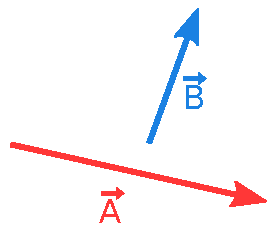
\includegraphics[scale=0.8]{Graphics/vectors/adding1}

Move them together head-tail and draw the sum as the vector between the ``total tail'' and ``total head'':
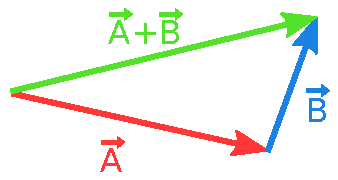
\includegraphics[scale=0.9]{Graphics/vectors/adding2}

This method works equally well with any number of vectors - just link them up tail-head as above; the sum vector will be the vector from the tail of the ``group'' to the head of the group, exactly as above.\\
The reason that we can do this is that vectors are completely characterized by their magnitude and direction - location in space is irrelevant. Two vectors with the same magnitude and direction are always equal, irrespective of their location. Therefore, we can move the vectors around to help us visualize vector addition.

So why does this method work? Well, imagine first traveling along $\vec{A}$, and then along $\vec{B}$. You would end up at $\vec{A}$ + $\vec{B}$. It really is that simple!

As for subtraction, one way to think about it is to \emph{add} the \emph{negative} vector instead, i.e. $\vec{a} - \vec{b} = \vec{a} + (-\vec{b})$. So what is $-\vec{b}$, exactly? It's simply the vector $b$ with the direction reversed. The magnitude is the same; the only difference is that you draw the arrow on the opposite side of the line.

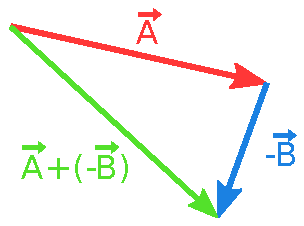
\includegraphics[scale=0.9]{Graphics/vectors/vectorsub}

Note that the vectors in the above graphic are the same vectors as in the addition example; however, the blue vector graphic is now $-\vec{b}$, which is then added to $\vec{a}$ to produce the result $\vec{a} - \vec{b}$.

That covers the basics of the graphical way to add and subtract vectors; what about the mathematical way? Well, in order to cover that, we need to first introduce the concept of vector components, and \emph{vector decomposition}.

What happens if we multiply a vector by a scalar (a dimensionless number)? Well, vectors work like numbers in that regard, in that $2 \cdot \vec{a} = \vec{a} + \vec{a}$. Draw that addition out on paper, and you'll see that the geometrical meaning is that the magnitude doubles, but the direction is unchanged.\\
As we saw above, when multiplying by negative numbers, the magnitude changes as appropriate, but the direction is flipped. $-3 \cdot \vec{a}$ would be a vector that is three times a big as $\vec{a}$, but points in the opposite direction. Multiplication by fractions (and even irrationals) work just as well, too.

\section{Vector components}

We can represent a vector as the sum of multiple vectors. In the most useful case, we can represent it as the sum of one vector ``per dimension'' the vector requires.\\
For a 2D vector in the Cartesian coordinate system, we can break a vector $\vec{A}$ into two vectors $\vec{A_x}$ and $\vec{A_y}$, such that the two vector components' directions are perpendicular; $\vec{A_x}$ points along the positive $x$ axis, while $\vec{A_y}$ points along the positive $y$ axis.

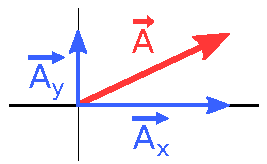
\includegraphics[scale=1.0]{Graphics/vectors/vectorcomponents}

Imagine moving $\vec{A_y}$ to the head of $\vec{A_x}$; if we draw the sum vector, we would get exactly $\vec{A}$. That is, $\vec{A} = \vec{A_x} + \vec{A_y}$.

We can also think of the magnitude of the partial vectors, $A_x$ and $A_y$. Those magnitudes represent how long the vector is in each dimension separately, and are very useful - more useful than the partial vectors themselves.

So \emph{why}, or where, is this useful? For one, when this technique is combined with unit vectors (below), it makes mathematical manipulation of vectors much easier. Vector decomposition can also be a powerful tool in solving physics problems, as it can break down problems in multiple dimensions to multiple smaller, one-dimensional problems, which are often easier to solve.

%\newpage

\subsection{Unit vectors}
Unit vectors are simple, but the concept is still very powerful. We define unit vectors to be vectors of magnitude 1 that point in the direction of their respective axes. The unit vector $\hat{i}$ (``i-hat``), points in the positive $x$ direction, while $\hat{j}$ points in the positive $y$ direction, and $\hat{k}$ in the positive $z$ direction. These unit vectors are also sometimes known as $\hat{x}$, $\hat{y}$ and $\hat{z}$, respectively. In addition, the ``hat'' suffix is sometimes called ``roof'', as in ``x roof''.

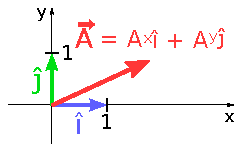
\includegraphics[scale=1.6]{Graphics/vectors/unitvectors}

Let's go back to the vector components above. The two components of $\vec{A}$ are both vectors, $\vec{A_x}$ and $\vec{A_y}$. We can write these components as the product of their magnitude (a scalar) and the unit vector in that direction (which is obviously a vector). Let's call the magnitude of vector $\vec{A_x}$  simply $A_x$.\\
Think of the vector $\vec{A_x}$ in the vector components figure as a longer version of the unit vector $\hat{i}$ - that is, it's the result of scalar multiplication of a magnitude, $A_x$, and the unit vector $\hat{i}$: $\vec{A_x} = A_x \hat{i}$\\
The same can be said for the component vector $\vec{A_y}$, which can be written as $A_y \hat{j}$.

Since we know that the sum of these two vectors equal $\vec{A}$, we now have
\[ \vec{A} = \vec{A_x} + \vec{A_y} \]
\[ \vec{A_x} = A_x \hat{i} \]
\[ \vec{A_y} = A_y \hat{j} \]
\[ \vec{A} = A_x \hat{i} + A_y \hat{j} \]

We have now written vector $\vec{A}$ as the sum of two separate, one-dimensional vectors. If we are working on a two-dimensional projectile motion problem, we can now calculate the motion along the x-axis as one problem, then calculate the motion along the y-axis as a separate problem, and then add the two together to get the combined motion. Doing so is generally much easier than solving the two-dimensional problem as-is.

We can also write that last equation ($\vec{A} = A_x \hat{i} + A_y \hat{j}$) as
\[ \vec{A} = \langle A_x, A_y \rangle \]
Here, we use a more compact notation, where the x and y components are listed, with the implicit meaning that me can construct the vector $\vec{A}$ by multiplying them by their respective unit vector, and adding the results.

%\newpage

\subsection{Vector decomposition}
Now that we know about vector components and unit vectors, let's apply these concepts, and also see how to actually do this decomposition mathematically. We've yet to see it from anything but a geometrical perspective. Sure, such perspectives are very useful for intuition, but in return, they are mostly useless for precise computation.\\
We can still use a picture to easier understand the mathematical decomposition, though:

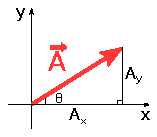
\includegraphics[scale=2]{Graphics/vectors/vectordecomp_trig}

Here, we see that $A_x$, $A_y$ and $\vec{A}$ form a right triangle.

Via the Pythagorean theorem, we see that
\[ |\vec{A}| = \sqrt{{A_x}^2 + {A_y}^2} \]

That is, the magnitude of the vector $\vec{A}$ is given by the sum of the squares of the component magnitudes.

If the vector were three-dimensional, we would simply add a ``$+ {A_z}^2$'' under the square root; the same goes for even higher dimensions.

However, while that is extremely useful, it doesn't help us \emph{find} $A_x$ and $A_y$ to begin with!\\
Let's stop stalling. Again, note how the three lines (if we consider the vector a line for now) form a right triangle. If we know the magnitude of the vector, i.e. the length of the hypotenuse, and the angle $\theta$ (theta) between the vector and the positive x axis, we can use trigonometry to find the components:

\[ \cos{\theta} = \frac{A_x}{|\vec{A}|} \]
\[ \sin{\theta} = \frac{A_y}{|\vec{A}|} \]

These come from the definitions of the sine and cosine functions - the cosine is the adjacent side ($A_x$) over the hypotenuse (the magnitude of $\vec{A}$), while sine is opposite ($A_y$) over hypotenuse.\\
We can now simply solve these equations for the components by multiplying both sides (of both equations) by the magnitude:

\[ A_x = |\vec{A}| \cos{\theta} \]
\[ A_y = |\vec{A}| \sin{\theta} \]

\subsection{Example}
Consider a vector with length/magnitude $|\vec{A}| = 5$ meters and angle $\displaystyle \theta = 30^{\circ} = \frac{\pi}{6}$ radians from the x axis. In other words, it's pointing ``to the right'' and slightly upwards, as seen from the origin.\\
In order to write this as a set of components, we can simply calculate the components as above:

\[ A_x = 5 \cos{\left( \frac{\pi}{6}\right) } = \frac{5 \sqrt{3}}{2} \approx 4.33 \text { meters} \]
\[ A_y = 5 \sin{\left( \frac{\pi}{6}\right) } = 2.5 \text { meters} \]

We can therefore write the vector as either of these forms (keeping in mind that we rounded the x value):
\[ \vec{A} = 4.33 \hat{i} + 2.5 \hat{j} \]
\[ \vec{A} = \langle 4.33, 2.5 \rangle \]

\section{Vector addition and subtraction, continued}
We now know what we need in order to talk about the mathematical way of vector addition and subtraction. Thankfully, once we've separated a vector into its components, addition and subtraction becomes incredibly easy!

Let's take the example of adding two vectors:
\[ \vec{a} = 5 \hat{i} + 3 \hat{j} \]
\[ \vec{b} = 2 \hat{i} - 1 \hat{j} \]
\[ \vec{a} + \vec{b} = (5 \hat{i} + 3 \hat{j}) + (2 \hat{i} - 1 \hat{j}) \]
\[ \vec{a} + \vec{b} = 7 \hat{i} + 2 \hat{j} \]

Yes, it's that easy - just add the parts separately, and you have the answer. Subtraction works as you would expect at this point. Let's try the more compact notation; the vectors used are the same as the ones in the addition example above.
\begin{align*}
\vec{a} = \langle 5, 3 \rangle\\
\vec{b} = \langle 2, -1 \rangle
\end{align*}
\begin{align*}
\vec{a} - \vec{b} &= \langle 5 - 2, 3 - (-1) \rangle\\
\vec{a} - \vec{b} &= \langle 2, 4 \rangle
\end{align*}

\section{The dot product / scalar product}
Now that we have addition and subtraction down, let's have a look at vector multiplication. There are two ways to multiply two vectors: the dot product, and the cross product.\\
The dot product gives a scalar result (a single number), and is therefore sometimes called the \emph{scalar product}, while the result of a cross product is a third vector.
Note that the two aren't simply different ways of doing the same thing, but fundamentally different operations, with completely different meanings and results.\\
The dot product is usually considered easier, so let's tackle that one first.

First off, notation. The name dot product comes from the notation used for the operation:
\[ \vec{a} \cdot \vec{b} \]

Before explaining the purpose of the dot product, let's go with the definitions and an example. It's rather easy to calculate, at least when you have the vector components.

Two definitions of the dot product, for two vectors with components $\vec{a} = \langle a_1, a_2, a_3 \rangle$ and $\vec{b} = \langle b_1, b_2, b_3 \rangle$, are:
\[ \vec{a} \cdot \vec{b} = a_1 b_1 + a_2 b_2 + a_3 b_3 \]
\[ \vec{a} \cdot \vec{b} = |\vec{a}| |\vec{b}| \cos{\theta} \]
Or, generally, for a vector with $n$ components/$n$ dimensions:
\[ \vec{a} \cdot \vec{b} = \sum_{i=1}^n a_i b_i = a_1 b_1 + a_2 b_2 + \cdots + a_n b_n \]

Let me just add one last definition before we look at this from a geometrical point of view:

\[ \vec{a} \cdot \vec{a} = |\vec{a}|^2 \]

Keeping in mind that the angle between a vector and itself must be 0, and that $\cos{(0)} = 1$, this should make sense if you believe the formulas above.

Therefore, the magnitude of a vector can also be written as:
\[ |\vec{a}| = \sqrt{\vec{a} \cdot \vec{a}} \]

Like vector addition, the dot product operation is commutative; that is, $\vec{a} \cdot \vec{b} = \vec{b} \cdot \vec{a}$. As we'll see later, however, the same is \emph{not} true for the cross product!

Now, if you've never seen the dot product before, I would assume you are a bit confused at this point. No worries - the above is meant as a ``reference'', not a tutorial. Let's get to the geometrical interpretation.

\subsection{Geometrical interpretation of the dot product}
Let's repeat the second definition of the dot product from above:
\[ \vec{a} \cdot \vec{b} = |\vec{a}| |\vec{b}| \cos{\theta} \]

Note that it's clear that the sign of the dot product is determined by (the cosine of) the angle and by that alone; the other terms are both magnitudes, which are always positive, by definition.\\
If the dot product is positive, the two vectors are pointing ``mostly'' in the same direction, i.e. the angle between them is less than 90 degrees; the angle is acute.
The dot product is zero if and only if the two vectors are perpendicular, as that's where the cosine term would be zero, and make the dot product zero as well.

%\newpage
And, if the angle is greater than 90 degrees, so that the vectors are pointing in different directions (with an obtuse angle between them), the dot product would be negative, as the cosine of the angle would be negative.

In a bit more concise form:
\[
\vec{a} \cdot \vec{b} =
	\begin{cases*}
	> 0 & \text{for $\theta < 90^\circ$, acute angle} \\
	  0 & \text{for $\theta = 90^\circ$, right angle} \\
	< 0 & \text{for $\theta > 90^\circ$, obtuse angle}
	\end{cases*}
\]

Now, let's look at this from a geometrical perspective, as promised.

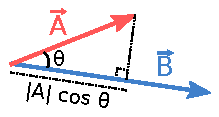
\includegraphics[scale=1.7]{Graphics/vectors/vectordot}

Here, we have two vectors, $\vec{A}$ and $\vec{B}$. We draw a line from $\vec{B}$, \emph{perpendicular} to $\vec{B}$, that meets $\vec{A}$ at the head. By definition, the angle between the line and $\vec{B}$ is 90 degrees.

Let's now use the definition of the cosine ($\displaystyle \cos \theta = \frac{\text{adjacent}}{\text{hypotenuse}}$) to find the length of the segment denoted by the dotted line, which we'll denote $|A_B|$, or ``the projection of $\vec{A}$ onto $\vec{B}$'':

\[ \frac{|A_B|}{|\vec{A}|} = \cos{\theta} \]
Solve for $|A_B|$ by multiplying both sides by the magnitude of $\vec{A}$:
\[ |A_B| = |\vec{A}| \cos{\theta} \]

Now we know, as the picture suggests, that the projection of $\vec{A}$ onto $\vec{B}$ is given by the magnitude of $\vec{A}$ times the cosine of the angle that separates the two vectors.\\
Now, remember the definition of the dot product:
\[ \vec{A} \cdot \vec{B} = |\vec{A}| \; |\vec{B}| \cos{\theta} \]
We can rearrange the terms to give:
\[ \vec{A} \cdot \vec{B} = |\vec{A}| \cos{\theta} \; |\vec{B}|\]
Using the identity just above, this is the same thing as:
\[ \vec{A} \cdot \vec{B} = |A_B| \; |\vec{B}|\]

So, we see that the geometrical interpretation of the dot product is, in one way to put it, the length that $\vec{A}$ goes in the direction of $\vec{B}$ (or the projection of $\vec{A}$ onto $\vec{B}$), times the magnitude of $\vec{B}$.\\
If this doesn't quite make sense, it will probably be easier to grasp when in actual use, such as when multiplying a force vector with a displacement vector to find work.

Another way (the same way, really) to think about it is this: imagine that the vector $\vec{B}$ is horizontal, i.e. parallel with the x axis, pointing to the right (the positive x axis).\\
Now, $|A_B|$ is just the x component of $\vec{A}$! Therefore, in general, we can think of $|A_B|$ as the ``B direction component'' of $\vec{A}$, so the dot product is the ``B direction component'' of $\vec{A}$ times the magnitude of $\vec{B}$.

\section{The cross product / vector product}
As the second naming suggests, this method of multiplying two vectors yields a third vector, namely one that is perpendicular to BOTH the vectors multiplied.\\
The notation used is, as the \emph{first} naming suggests, a cross:
\[ \vec{A} \times \vec{B} = \vec{C} \]

The cross product is only properly defined for 3- and 7-dimensional vectors. We will of course only work with the former in this course.

Okay, so we know that the cross product gives a third vector, that is perpendicular to both the vectors multiplied. It's also very important to know that the cross product operator is not commutative. That is,

\[ \vec{B} \times \vec{A} \neq \vec{A} \times \vec{B} \]
It is \emph{anti-commutative}:
\[ \vec{B} \times \vec{A} = -(\vec{A} \times \vec{B}) \]

It also works alongside scalar multiplication, so that
\[ (r \vec{A}) \times \vec{B} = \vec{A} \times (r \vec{B}) = r(\vec{A} \times \vec{B}) \]

Okay, okay, enough with the side-definitions. What is the definition of the cross product?\\
Well, as previously, there are two definitions we'll use: one that uses magnitude and angle, and one that uses vector components. The latter is rather complex, but here's the first one, to begin with: \subsection{Definition: Magnitude and angle}

\[ \vec{A} \times \vec{B} = |\vec{A}| \; |\vec{B}| \; \sin{\theta} \; \hat{n} \]
This is, you might note, very similar to the dot product, except it has a sine rather than a cosine, and also has a direction (we'll get to that soon), since it's a vector.\\
If we want just the magnitude of the cross product, it's eerily similar to the dot product:
\[ |\vec{A} \times \vec{B}| = |\vec{A}| \; |\vec{B}| \; \sin{\theta} \]
The sine instead of the cosine is now the only difference.

One way to think about it is that the \emph{dot} product measures ``how parallel'' two lines are. When completely parallel, the dot product is at its maximum. (Mathematically, the $\cos{\theta}$ term is 1, its maximum, when $\theta = 0$, i.e. the angle between the two is 0, i.e. they are completely parallel.)\\
The dot product is then zero when the vectors are perpendicular (not parallel at all), and negative when they point in different directions ($\theta > 90^\circ$).

What about the \emph{magnitude of} the cross product (not just the cross product itself!)? It's pretty much the opposite: you can think of it as measuring ``how perpendicular'' two vectors are. With two fully parallel vectors, the cross product equals zero (the angle $\theta = 0$, and $\sin{(0)} = 0$). When they are perpendicular, the cross product is at its maximum, since $\sin{(90^\circ)} = 1$.

Okay, so that covers the magnitude, what about the direction, $\hat{n}$? As the hat/roof suggests, that is a unit vector... but in what direction? Hang on; we'll discuss that in the geometrical interpretation, after the component definition.

\subsection{Definition: components}

The second definition, using components - in its worst possible form (it'll get better soon) - is:
\[ \text{For } \vec{C} = \vec{A} \times \vec{B}\text{:} \]
\[ \vec{C} = (A_y B_z - A_z B_y) \hat{i} + (A_z B_x - A_x B_z) \hat{j} + (A_x B_y - A_y B_x) \hat{k} \]
Oh dear. Thankfully, there are ways to remember the above. First, what we do - for the mnemonic to work - is to rename the variables, and instead compute
\[ \vec{A} = \vec{B} \times \vec{C} \]
Without this change, the mnemonic is probably \emph{harder} to remember than the above mess, so go with me.\\
After that change, we write the component equations separately, instead of all on one line. The sums-of-products are the same as above, though, if we account for the variable renames:
\[ A_x = B_y C_z - B_z C_y \]
\[ A_y = B_z C_x - B_x C_z \]
\[ A_z = B_x C_y - B_y C_x \]

Still awful. Heck, it might just look harder like this! Don't panic - there's a pattern: {\bf XYZZY}.\\
Note that the subscripts of the first equation spell XYZZY, and that the vector order is alphabetical for all equations ($A_* = B_* C_* - B_* C_*$).\\
That makes the first one relatively easy (compared to memorizing the entire thing), but what about the rest?\\
A-ha! Here's the pattern: to convert from the first equation to the second, ``increase'' the subscript by one letter; if at z, go back to x. That is, $A_x$ becomes $A_y$ (one letter ahead), $A_y$ becomes $A_z$ (one letter ahead), and $A_z$ wraps around and becomes $A_x$; the same thing applies to the B and C components.\\
The same method is used to convert from the second to the third equation. Have a close look at them and make sure you realize this is true!

As an additional sanity check, note that the reverse of the first subscript pair is the one you then subtract: yz - zy, zx - xz and xy - yx. (Look at the subscripts in the three equations again if you don't get what I mean.)

Since $\vec{C}$ is supposed to be perpendicular to both $\vec{A}$ and $\vec{B}$, we can use the dot product to check whether our answer appears to be correct or not. Remember that the dot product is always zero for two perpendicular vectors - so we could check our work by testing that the two dot products $\vec{A} \cdot \vec{C}$ and $\vec{B} \cdot \vec{C}$ are both zero. If either or both is \emph{not} zero, the cross product calculation was done incorrectly. If both \emph{are} zero, that doesn't guarantee that the answer is correct, however. More on that later (there are two vectors perpendicular to both $\vec{A}$ and $\vec{B}$: $\vec{C}$ and -$\vec{C}$).

%\newpage
\subsection{Geometrical interpretation of the cross product}
Let's try to make sense of all the above.\\
We can imagine a parallelogram plane in 3D space, with two sides $\vec{A}$ and $\vec{B}$. This is certainly one of those times where an image is worth (more than) a thousand words:

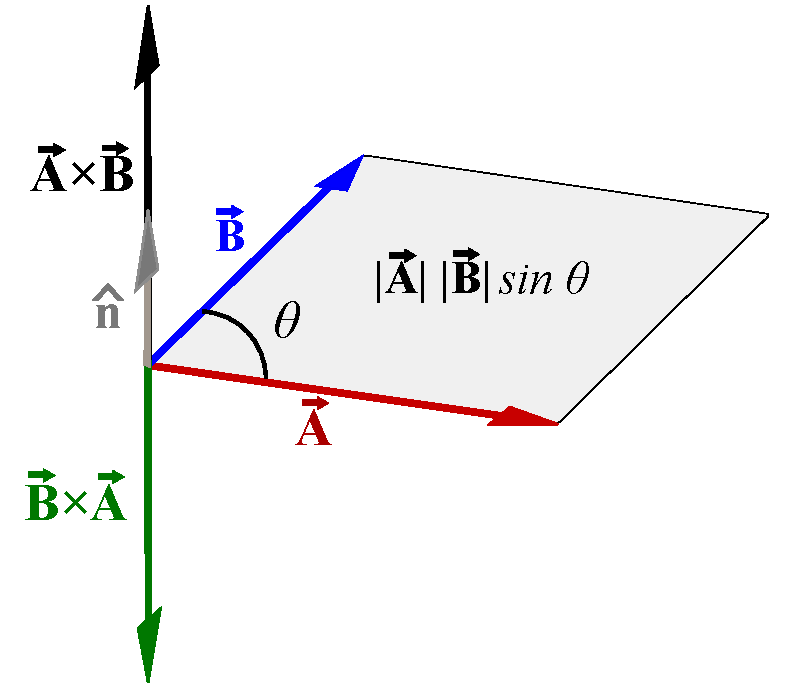
\includegraphics[scale=0.5]{Graphics/vectors/cross-product-with-area}

(Image license is CC0. By Wikimedia user Svjo; modified by me.)

Here, we can see several key things:
\begin{itemize*}
\item The area of the parallelogram is the magnitude of the cross product, $|\vec{A}| \; |\vec{B}| \; \sin{\theta}$ (this is one of the ways to calculate the area of a parallelogram).
\item The unit vector $\hat{n}$ (and therefore the cross product) is indeed perpendicular to \emph{both} $\vec{A}$ and $\vec{B}$; another way of saying this is that it's perpendicular to the plane formed by $\vec{A}$ and $\vec{B}$.)
\item $\vec{B} \times \vec{A}$ points in the opposite direction as $\vec{A} \times \vec{B}$ does, since $\vec{B} \times \vec{A} = -(\vec{A} \times \vec{B})$. (Remember that the negative of a vector is a vector pointing in the opposite direction, i.e. with the arrowhead on the other side of the line.)
\end{itemize*}

However, we also see a problem: if both the upwards-pointing vector $\vec{A} \times \vec{B}$ and the downwards-pointing vector $\vec{B} \times \vec{A}$ are perpendicular to both $\vec{A}$ and $\vec{B}$, and they are (obviously!) not equal... how do we know which of the two to use? How do we identify which is which?

We'll have to use a rule known as the \emph{right-hand rule} for this.\\
The right-hand rule is often taught in different ways, all with the same end result. The way I prefer is one using your whole right arm, simply because because I find it easier.\\
The rule is this: if your entire right arm points along the first vector ($\vec{A}$), angle your index through pinky (four fingers) in the direction of the second vector ($\vec{B}$); if this means you have to turn your arm, do so.\\
Now, with your arm pointing along vector $\vec{A}$ and your fingers pointing along vector $\vec{B}$, extend the thumb straight out. Your thumb should now be perpendicular to both $\vec{A}$ and $\vec{B}$, and point along $\vec{A} \times \vec{B}$ (and not $\vec{B} \times \vec{A}$ - try swapping the arm and the finger vectors, and you'll find that the result is the thumb pointing in the opposite direction!).

That is:

\begin{itemize*}
\item Right hand/entire arm points parallel to $\vec{A}$
\item Fingers are curled to point parallel to $\vec{B}$
\item Thumb now points parallel to $\vec{A} \times \vec{B}$ (perpendicular to both $\vec{A}$ and $\vec{B}$).
\end{itemize*}

Note that this is only true for certain coordinate systems, namely \emph{right-handed} ones. These are the ones used by all sane persons in physics, and the only ones used in this document.

One useful definition to test whether a system is right-handed or not, is that this SHOULD be true:

\[ \hat{i} \times \hat{j} = \hat{k} \]
If the above is false for your coordinate system (i.e. you get $-\hat{k}$ instead), your coordinate system is left-handed and simply won't work according to the definitions generally used in physics!

\end{document}